\documentclass{article}

%Вставки кода
\usepackage{listings} 

%добавляет русский язык
\usepackage[english,russian]{babel}
\usepackage[14pt]{extsizes}
%Рисунки
\usepackage[dvips]{graphicx}
%Каталоги для рисунков
\graphicspath{{./image-parallel/}{image-git/}}
%Пакет работы с цветом
\usepackage{color}
\definecolor{mygreen}{rgb}{0,0.6,0}
\definecolor{mygray}{rgb}{0.5,0.5,0.5}
\definecolor{myorange}{rgb}{1,0.5,0.25}
%Пакет работы с гиперссылками и установка цвета ссылок
\usepackage[colorlinks,linkcolor=blue,urlcolor=blue]{hyperref}
%Отступы
\usepackage[left=3cm,right=2cm,top=2cm,bottom=2cm,bindingoffset=0cm]{geometry}
%Добавление абзацев после оглавления (indentfirst)
\usepackage[indentfirst]{titlesec}
\usepackage{titletoc}
%%TODO Настроить нумерацию
\usepackage[utf8]{inputenc}
\linespread{1.3}
%Для таблиц
\usepackage{multirow}
\author{Морозов С.Д.}
\begin{document}

%Настройка параметров вставок кода

\lstset{ 
	language=C,                 % выбор языка для подсветки (здесь это С)
	basicstyle=\small\sffamily, % размер и начертание шрифта для подсветки кода
	numbers=left,               % где поставить нумерацию строк (слева\справа)
	stepnumber=1,                   % размер шага между двумя номерами строк
	numbersep=5pt,                % как далеко отстоят номера строк от подсвечиваемого кода
	backgroundcolor=\color{white}, % цвет фона подсветки - используем \usepackage{color}
	keywordstyle=\color{blue},	
	showspaces=false,            % показывать или нет пробелы специальными отступами
	showstringspaces=false,      % показывать или нет пробелы в строках
	showtabs=false,             % показывать или нет табуляцию в строках
	frame=single,              % рисовать рамку вокруг кода
	tabsize=2,                 % размер табуляции по умолчанию равен 2 пробелам
	captionpos=t,              % позиция заголовка вверху [t] или внизу [b] 
	breaklines=true,           % автоматически переносить строки (да\нет)
	breakatwhitespace=false, % переносить строки только если есть пробел
	escapeinside={\%*}{*)},   % если нужно добавить комментарии в коде
	numberstyle=\tiny\color{mygray},
  	rulecolor=\color{black},
  	stringstyle=\color{myorange},
  	commentstyle=\color{mygreen},
}


\begin{titlepage}
	\centering
	{\LARGE Университет ИТМО \par}
	\vspace{5mm}
	{\Large Кафедра вычислительной техники\par}
	\vspace{1.5cm}
	{\huge\bfseries Отчет по прохождению практики\par}
	\vspace{3cm}
	\begin{flushleft}
		\hangindent=10cm
		\hangafter=-5
		\noindent 
		{\Large Студента\\
				P3311 группы \\
				Морозова С.Д.\\
				Руководитель \\
				Соснин В.В.
		}
	\end{flushleft}
	\vfill
% Bottom of the page
	\vspace{1cm}
	{\large Санкт-Петербург \par}
	{\large 2016  \par}
\end{titlepage}
%Нужны ли в содержании subsubsection'ы?
	\setcounter{tocdepth}{3}	
	\tableofcontents
	\newpage
	\section{Введение}
	\indent 
	%%Тема паралельные вычисления. Перед тем как приступить к тебе необходимо разобраться с латех и гит...
		Тема прохождения практики "--- параллельные вычисления. Цель задания "--- сравнить различные функции в языке С, которые 		можно использовать для измерения времени работы параллельных программ.
		
		Однако требования руководителя практики таковы, что перед тем как приступить к выполнению основного задания нужно 				ознакомиться с системой компьютерной вёрстки TeX (LaTeX), которая должна
	использоваться для написания отчёта, и ознакомиться с системой контроля версий Git, с последующим созданием учетной записи на 	сайте GitHub или анагичном.
	\newpage
	\section{Система компьютерной верстки \TeX(\LaTeX)}	
		\subsection{Краткое описание}
			\TeX ~"--- система компьютерной вёрстки с формулами, разработанная американским профессором информатики Дональдом 				Кнутом. Название происходит от греческого слова $\tau\varepsilon\chi\upsilon\eta$ "--- "<искусство">, "<мастерство">, 				поэтому	последняя буква читается как русская Х. Хотя TeX является системой набора и верстки, развитые возможности 					макроязыка TeX делают его Тьюринг-полным языком программирования. 
		
			\TeX ~работает с боксами (box) и клеем (glue). Бокс "--- двумерный объект прямоугольной формы, характеризуется тремя 
		величинами (высота, ширина, глубина). Элементарные боксы "--- это буквы, которые объединяются в боксы-слова, которые в 				свою очередь сливаются в боксы-строчки, боксы-абзацы и т.д.

        	Между боксами располагается клей, который имеет некоторую ширину по умолчанию и степени увеличения/уменьшения этой 				ширины. Объединяясь в бокс более высокого порядка, боксы могут шевелиться, но после того как найдено оптимальное решение, 		это состояние закрепляется, и полученный бокс выступает как единое целое.
        
       		Инетересный факт. На версии 3.0 дизайн был заморожен, поэтому в новых версиях не будет добавления новой 						функциональности, только исправление ошибок. Версия \TeX 'a ассимтотически приближается к числу $\pi$. Это факт говорит о 		том, что последняя версия	3.14159265 (январь 2014) является крайне стабильной и возможны лишь мелькие исправления. 				Дональд Кнут заявил, что последнее обновление (сделанное после его смерти) сменит номер версии на ~$\pi$, и с этого 				момента все ошибки станут особенностями.
        		
			\LaTeX ~"--- созданный Лесли Лэмпортом набор макрорасширений (или макропакет) системы компьютерной вёрстки \TeX, 				который облегчает набор сложных документов. Стоит отметить, что как и любой другой макропакет\footnote{ Так же существуют 		Plain TeX, AMS-TeX, AMS-LaTeX и т.д.} \LaTeX ~не может расширить возможности \TeX ~(все, что можно сделать в одном пакете 		можно сделать и в любом другом). Пакет позволяет автоматизировать многие задачи набора текста и подготовки статей, 					включая набор текста на нескольких языках, нумерацию разделов и формул, размещение иллюстраций и таблиц на странице, 				ведение библиографии и др. Все это делает \LaTeX ~крайне удобным инструментом для написания научных статей, диссертаций и 		т.п..
					
		\subsection{Сравнение \LaTeX ~и MS Word}
			В качестве сравнения "--- перечислим плюсы и минусы \LaTeX ~перед MS Word(а так же всеми его аналогами). \\	
	    Плюсы \LaTeX: 
	    \begin{itemize} 
	    	%\item	Проста работы с любыми математическими формулами
	    	\item	Кроссплатформенность 
	    	%\item	Без особых трудностей можно получить сноски, список литературы,
			%		оглавление, список таблиц, указатель и т. п.
	    	%\item	Имеется несколько стандартных стилей (книга, статья, доклад,
			%		письмо), с помощью которых получаются документы очень высокого
			%		полиграфического качества 
	    	%\item	Гибкая работа с логической структурой текста
	    	\item	Язык международного обмена по математике и физике (большинство     
   					научных издательств принимают тексты в печать  только в этом формате)
    	\end{itemize}
    Минусы \LaTeX:
		\begin{itemize} 
	    	\item	Не является системой типа WYSIWYG
	    				\footnote{What You See Is What You Get(Что видишь, то и получишь). Стоит отметить, что существуют 									дистрибутивы \TeX ~в которых есть попытки реализовать WYSIWYG. Например платный дистрибутив  BaKoMa TeX + 						текстовый редактор  BaKoMa TeX Word.}   
	    	\item	При серьезных отклонениях от стандартных стилей документов требуется
					достаточно сложное программирование	
    	\end{itemize}
    	
    		То есть, выбирая между \LaTeX ~и MS Word, стоит обратить внимание на то,какой текст вы собираетесь печатать, 					насколько нестандартный будет стиль текста, на его примерный объем. В некоторый случаях достаточно использовать MS Word,   		в других "--- использование \LaTeX ~может заметно упростить работу.
		\newpage		
		\subsection{Выбор инструмента редактирования}
			В ходе изучения всех возможных вариантов работа с \LaTeX ~для создания данного отчета, была выбрана программа 						Textmaker
			\footnote{Оффициальный сай Textmaker:~ \href{http://www.xm1math.net/texmaker/}{http://www.xm1math.net/texmaker/}}.\\
			Выбор Textmaker'а обусловлен следующими его особенностями:
			\begin{itemize} 
	    		\item	Автоматическая подсветка синтаксиса
	    		\item	Функция автодополнения команд \LaTeX
	    		\item	Сокрытие блоков кода (Code folding)
	    		\item	Быстрая навигация по структуре документа
	    		\item	Указание на строку с ошибкой, для быстрой отладки
	    		\item	Интегрированный просмотр PDF
			\end{itemize} 
	\newpage
	\section{Системы контроля версий}
		\subsection{Краткое описание}
			Система контроля версий (СКВ) — это система, регистрирующая изменения в одном или нескольких файлах с тем, чтобы в 				дальнейшем была возможность вернуться к определённым старым версиям этих файлов. 
				
			СКВ широко используются при разработке программного обеспечения, для хранения кодов разрабатываемых программ. Однако 			данные системы подходят не только программистам. Художники, которые хотят сохранять каждое изображение/эксиз своей 					работы, писатели пишущие книги или научные статьи, бухгалтеры, которые хранять разные версии отчетов и т.д., все они 				могут использовать СКВ для достижения своих целей.
				
			Иначе говоря СКВ можно применять в любых областях в которых ведётся работа с большим количеством непрерывно 					изменяющихся электронных документов.
		\subsection{Git}
			Git "--- созданная Линусом Торвальдсом, распределенная система контроля версий.
			\subsubsection{Особенности}
			% По большей части взято от сюда -> https://git-scm.com . Позже может быть перепишу своими словами.  
				Одной из основных особенностей Git состоит в способе хранения данных. В принципе, большинство других систем 					хранит 	информацию как список изменений (патчей) для файлов. Эти системы (CVS, Subversion, Perforce, Bazaar и другие) 			относятся к хранимым данным как к набору файлов и изменений, сделанных для каждого из этих файлов во времени, как 					показано на Рис.~\ref{ris:other-scv}
			
			\begin{figure}[h!]
				\center{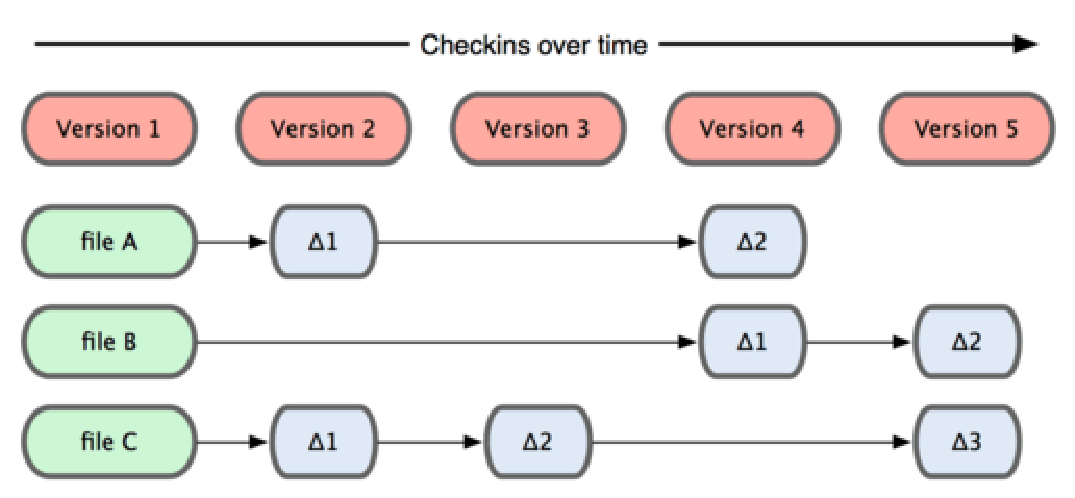
\includegraphics[width=0.80\linewidth]{other-scv}}
				\caption{Другие системы хранят данные как изменения к базовой версии для каждого файла.}
				\label{ris:other-scv}
			\end{figure}	
			\newpage
				Git не хранит свои данные в таком виде. Вместо этого Git считает хранимые данные набором слепков небольшой 						файловой системы. Каждый раз, когда вы фиксируете текущую версию проекта, Git, по сути, сохраняет слепок того, как 					выглядят все файлы проекта на текущий момент. Ради эффективности, если файл не менялся, Git не сохраняет файл снова, 				а делает ссылку на ранее сохранённый файл. То, как Git подходит к хранению данных, похоже на Рис.~\ref{ris:git}
			
			\begin{figure}[h!]
				\center{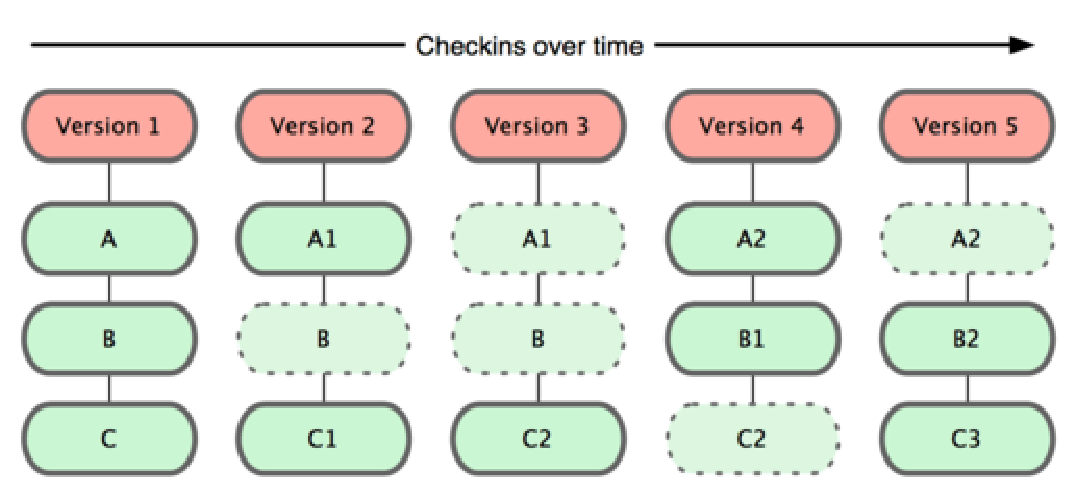
\includegraphics[width=0.80\linewidth]{git}}
				\caption{Git хранит данные как слепки состояний проекта во времени.}
				\label{ris:git}
			\end{figure}
			\newpage
				За счет этого, для большинства операций в Git нужны только локальные ресурсы и файлы. Что в свою очередь 						определяет два основных преимущества Git перед остальными СКВ.
			\begin{itemize}
	    		\item	Быстродействие. Поскольку вся история проекта хранится локально у вас на диске, большинство операций 							кажутся практически мгновенными(в отличии от централизованных системам, где практически на каждую операцию 							накладывается сетевая задержка).
	    		\item	Возможность работать(делать коммиты) без доступа к сети или VPN.
			\end{itemize}
			\newpage
			\subsubsection{Основные команды}
			В целом, следующая картинка (Рис.~\ref{ris:git-command}) наглядно демонстрирует основные команды Git, знание которых 			достаточно, чтобы начать им пользоваться.
			
		\begin{figure}[h]
			\center{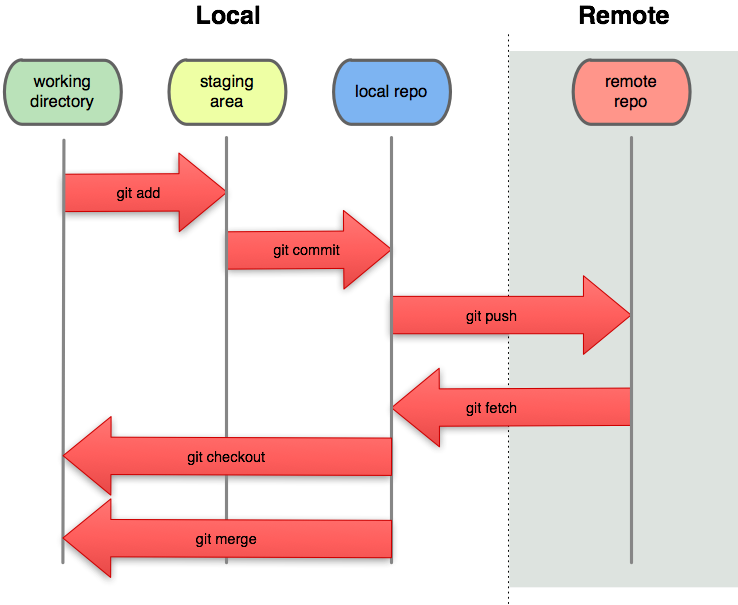
\includegraphics[width=0.75\linewidth]{git-command}}
			\caption{Основные команды при работе с Git.}
			\label{ris:git-command}
		\end{figure}
		\newpage
		\subsection{GitHub}
			\href{https://github.com/}{GitHub} — крупнейший веб-сервис для хостинга IT-проектов и их совместной разработки. 				Основан на системе контроля	версий Git и разработан на Ruby on Rails и Erlang компанией GitHub, Inc (ранее Logical 					Awesome).
			
			В ходе прохождения практики, на сайте GitHub была создана учетная запись ~\href{https://github.com/MorozovSD}					{MorozovSD}. В данной учетной записи был создан репозиторий ~\href{https://github.com/MorozovSD/Practice-2016}						{Practice-2016} по которому можно легко отследить процесс прохождения практической работы.
	\newpage
	\section{Паралельные вычисления}
		Т.к. практика предполагает не доскональное изучение параллельного программирования, а лишь сравнение функций замера 			времени в программах, работающих на основе парралельных вычислений, то данная глава носит более ознакомительных характер, 			содержащий тот минимум знаний, необходимый для работы с этой области.
		\subsection{Немножко теории}
		%Интуит Академия Microsoft: Параллельные вычисления и многопоточное программирование разделения компьютеров на три 						класса:	
			%Мультипроцессорные вычислительные комплексы - это компьютеры, обладающие множеством процессоров, работающих на общей 			памяти. В этот класс входит большинство продаваемых сегодня на рынке многоядерных компьютеров.

			%Мультикомпьютерные вычислительные комплексы - представляют множество компьютеров, соединенных высокоскоростными 				линиями связи. Каждый компьютер обладает собственной памятью и обменивается сообщениями с другими компьютерами системы 				для передачи данных. 
	
			Мультипрограммирование "--- параллельное выполнение нескольких программ. Мультипрограммирование позволяет уменьшить 			общее время их выполнения.
			
			Под параллельными вычислениями понимается параллельное выполнение одной и той же программы. Параллельные вычисления 			позволяют уменьшить время выполнения одной программы. Чаще всего, хороший последовательный алгоритм не является таковым 			для параллельного выполнения.(а параллельные алгоритмы могут не являться эффективными при работе с одним процессором), 				поэтому одна из задач паралельных вычислений это разработка эффективных алгоритмов, полностью использующие количество 				преподставленных процессоров. 
			
			Т.к. тема практики "--- измерение времени работы пареллельно работаящей программы, то необходимо получить оценку    			времени выполения программы одним процессором $T_1$  для идеализированного случая, когда число процессоров не 						ограничивается "--- $T_\infty$. А так же оценить верхнюю и нижнюю границы времени выполнения конечным число процессоров 			$T_p$\footnote{В отчете будут представленны только конечные формулы, без доказательств}.
						
		Для введенных характеристик очевидно следующее соотношение:

		\begin{equation}
			\label{eq:easy_attetude}
			T_\infty \le T_p \le T_1
		\end{equation}
			
		Для $T_p$ справедлива следующая оценка снизу:
			
		\begin{equation}
			\label{eq:lower_bound}
			T_p \ge \frac{T_1}{p}
		\end{equation}
			
		Для $T_p$ справедлива следующая оценка сверху:
			
		\begin{equation}
			\label{eq:upper_bound}
			T_p \le \frac{T_1}{p} + T_\infty
		\end{equation}
			
		Исходя из вышеперечисленных неравенств, неравенство(\ref{eq:easy_attetude}) может быть заменено более точным:
			
		\begin{equation}
			\label{eq:attetude}
			\frac{T_1}{p} \le T_p \le \frac{T_1}{p} + T_\infty
		\end{equation}
			
		

		На графике это выглядит следующим образом (Рис.~\ref{ris:graph_attetude}):
			
		\begin{figure}[h!]
			\center{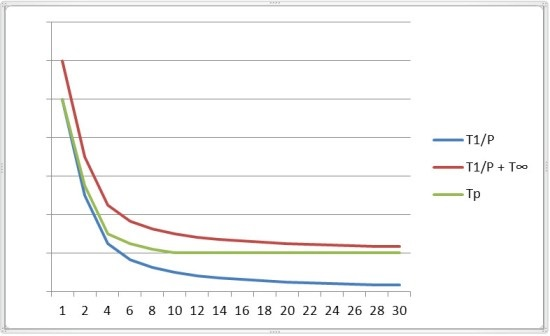
\includegraphics[width=1\linewidth]{graph_attetude}}
			\caption{Графическая интерпритация поведения функции $T_p$}
			\label{ris:graph_attetude}
		\end{figure}
						
			Очевидно, что при $p = 1$ графики функций $T_p$ и $\frac{T_1}{p}$ совпадают. Так же происходит совпадение графиков 				$T_p$ и $\frac{T_1}{p}+T_\infty$ при $p\to\infty$.
		\newpage
		\subsection{Характеристики параллельных вычислений}
			\subsubsection{Ускорение}
				Ускорение $S_p(n)$\footnote{Все вводимые характеристики рассматриваются как функции параметра $n$, 								характеризующего сложность решаемой задачи. Обычно $n$ понимается как объем входных данных.} определяют как 						отношение:
				
			\begin{equation}
				\label{eq:acceleration}
				S_p(n) = \frac{T_1(n)}{T_p(n)}
			\end{equation}			
				
				Интерпритировать данную формулу следует как отношение время наилучшего алгоритма, для которого достаточно одного 				процессора, и время наилучшего параллельного алгоритма, который может использовать $p$ имеющихся процессоров.				
				
			\subsubsection{Эффективность}
				Эффективность $E_p(n)$ определяют как отношение:
				
			\begin{equation}
				\label{eq:efficiency}
				E_p(n) = \frac{S_p(n)}{p}
			\end{equation}	

				При оптимальном ускорении\footnote{Оптимальное ускорение достигается когда $T_p = \frac{T_1}{p}$} эффективность 				равна 1. Если же эффективность существенно ниже 1, то часто число процессоров целесообразно уменьшить, используя 					их более эффективно. 
				
			\subsubsection{Упущенная эффективность}
				Мера неиспользованных возможностей "--- упущенной выгоды "--- $U(n)$, определяют следующим образом:
			
			\begin{equation}
				\label{eq:loss_of_efficiency}
				U(n) = \frac{T_p(n)}{T_{p_{opt}}} - 1
			\end{equation}
			
				Оптимальное время, которое можно достичь, используя $p$ процессоров, дается нижней оценкой для $T_p$, 							поэтому получаем:	

			\begin{equation}
				\label{eq:loss_of_efficiency_second}
				U(n) = p\frac{T_p(n)}{T_1} - 1
			\end{equation}
				
				Если для компьютера с $p$ ядрами время решения задачи оптимально и сокращается в $\sim p$ раз в сравнении с 					решением задачи на одноядерном компьютере, то наши потери равны нулю, возможности компьютера полностью используются. 				Если же задача решается за время $T_1$ "--- столь же долго, как на одноядерном компьютере, то потери пропорциональны 				числу неиспользованных ядер.
				
		\subsection{Основные проблемы паралельного программирования}
			\subsubsection{Синхронизация}
				Синхронизация нужна для того, чтобы согласовать обмен информацией между модулями (между параллельно выполняемыми 				множествами операций). Синхронизация может привести к простою процессора, т.к. после достижения точки синхронизации 				он должен ждать, пока другие задания достигнут точки синхронизации. Задержка с подачей в процессор необходимых данных 			ведет к простою процессора и снижению эффективности параллельной обработки
			\subsubsection{Гонка данных}
				Проблема "<гонки данных"> возникает для мультипроцессорных компьютеров с общей памятью. В одни и те же моменты 					времени процессоры могут получать доступ к одним и тем же данным,хранимым в общей памяти, как для чтения, так и для 				записи.
				
				Если с чтением данных проблем не возникает,то одновременная запись двух разных значений в одну и ту же ячейку 					памяти не возможна. Запись всегда идет последовательно, следовательно в памяти останется храниться значение, 						пришедшее последним (причем не известно какое значение каким прийдет). Конкурирование процессоров за запись в одну и 				ту же ячейку памяти и есть "<гонка данных">. 
				
				Один из способов справиться с этой проблемой "--- это закрытие доступа к ресурсу первым пришедшим процессором. 					Остальные процессоры прерывают выполнение и становятся в очередь за обладание ресурсом. Обладатель ресурса спокойно 				выполняет свою работу, а по ее окончании открывает ресурс, с которым теперь начинает работать тот, кто первым стоит в 			очереди.

				%Гонка данных "--- это одна из самых серьезных проблем параллельного программирования, поскольку при некорректно 				организованной блокировке ресурса программа может завершаться с некорректными результатами без возникновения 						исключительных ситуаций.
				
			\subsubsection{Взаимная блокировка (Deadlock)}
				Блокировка "--- хороший механизм решения проблемы "<гонки данных">. Однако блокировка может прервать выполнение 				всей программы, когда наступает ситуация, называемая взаимной блокировкой, клинчем, смертельным объятием или 						deadlock'ом.
				
				В качестве примера рассмотрим простейшую ситуацию, приводящую к возникновению клинча. Пусть есть два конкурента 				$A$ и $B$, претендующие на два ресурса $x$ и $y$. Пусть гонку за ресурс $x$ выиграл $A$ и соответственно закрыл этот 				ресурс для $B$. Гонку за ресурс $y$ выиграл $B$ и закрыл ресурс для $A$. Но $A$, чтобы закончить свою работу нужен 					ресурс $y$, поэтому он стал в очередь, ожидая освобождения ресурса. Симметрично, $B$ находится в очереди, ожидая 					освобождения ресурса $x$. Возникает ситуация вечного ожидания (которое может разрешить только внешнее воздействие), 				когда ни $A$, ни $B$ не могут продолжить свою работу.(Рис.~\ref{ris:deadlock}):
			
			\begin{figure}[h!]
				\center{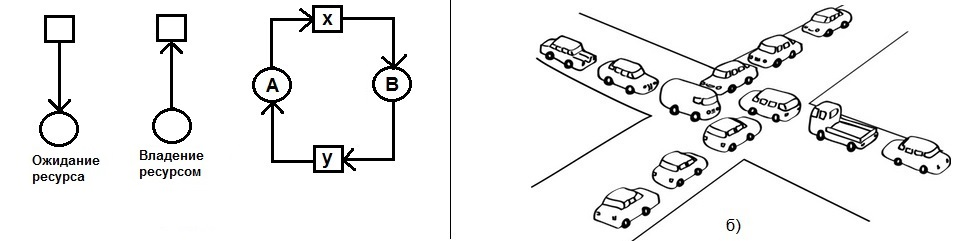
\includegraphics[width=0.80\linewidth]{deadlock}}
				\caption{Взаимная блокировка (клинч): а) Общий вид. б) На примере перекрестка.}
				\label{ris:deadlock}
			\end{figure}
	\newpage
			%\subsubsection{Проблема мультикомпьютерных комплексов}
		\subsection{Распарелеливание цикла}
		%http://www.intuit.ru/studies/courses/10554/1092/lecture/27091
			Думаю стоит перенести эту главу в практическую часть, и в ней предложить наиболее оптимальный параллельный алгоритм 			суммирования (т.к. тестовая программа решает задачу суммирования квадратов).
	\newpage
	\section{Функции замера времени}
		%Можно подробнее расписать типы данных и добавить tm и _SYSTEMTIME 
		%%Описывание разных функций замера времени
		Эта глава посвещена функциям замера времени языка Си.
		\subsection{Категории функций?}	
			Функции работы со временем можно отнести к трем категориям:
			\begin{itemize} 
				\item Функции календарного времени 
				\item Функции для измерения прошедшего времени CPU
				\item Функции для установки будильников и таймеров
					\footnote{Данная категория функций не используется в практической работе, и рассматриваться не будет}
			\end{itemize}
			\subsubsection{Календарное время}
				 Осуществляет для слежения за датами и временем согласно Грегорианскому календарю. Существуют несколько способов 				представления информации даты и времени. Т.к. нас интересует разрешающая способность (точность замеров времени) 					рассмотрим эти способы представления в зависимости от их разрешающей способности.
			\begin{itemize} 
				\item Тип данных time$\_$t "---  компактное представление, обычно дает число секунд, истекающих начиная с 								некоторого основного времени. Разрешающая способность одна секунда
				\item Тип данных struct timeval "--- представление времени с большей точностью. Разрешающая способность до 								микросекунд
					\footnote{На некоторых платформах возможно отслеживание времени только в пределах разрешающей способности 							системного таймера, который в общем случае устанавливается на значение 100 Гц}
				\item Тип данных timespec  "--- представление времени с большей точностью. Разрешающая способность до 									наносекунд
			\end{itemize}	 
			\subsubsection{Время процессора}
				Процессорное время отлично от фактических часов, тем что оно не включает временя выполнения другого процесса и 					все потраченное время на ожидание ввода-вывода. Процессорное время представляется типом данных clock$\_$t, и дано 					как ряд импульсов времени относительно произвольного базового времени
			\footnote{Для перевода количества импульсов в секунды, количество импульсов неоходимо делить на CLOCKS$\_$PER$\_$SEC 				(число	импульсов времени clock в секунду)}
			, отмечающего начало одиночного вызова программы. 
				
				В зависимости от архитектуры компьютера и операционной системы способ слежения за процессорным временем может 					быть разным. Общее для внутренних часов процессора то, что разрешающая способность где-то между тысячной и милионной 				долей секунды.
		
		%https://www.opennet.ru/docs/RUS/glibc/glibc-17.html
		\subsection{Функции}
		%clock_getres - узнать разрешающую способность
		%clock_gettime - запись системного времени в структуру
		%clock_settime - запись времени из а в б
		%целая куча виндовских функций в сприставкой _s
		%difftime  - разница между временем
		В данной главе будут описаны функциии замера времени в операционных системах Windows и Linux. 
		\subsubsection{Кроссплатформенные функции}
			\paragraph{clock}
				$$clock\_t~clock~(void)$$
				
				Функция возвращает прошедшее \underline{процессорное время}. Базовое время произвольно, но не изменяется внутри 				одиночного процесса. Если процессорное время не доступно или не может представляться, clock возвращает значение 					(clock$\_$t) (-1).
			\paragraph*{time}
				$$time\_t~time(time\_t~ *~ timeptr)$$
				
				Функция возвращает текущее \underline{календарное значение времени} в секундах. Если аргумент не является нулевым 			указателем, ей передается значение времени типа time$\_$t.
				
				
			\paragraph*{omp$\_$get$\_$wtime}
			$$double~omp\_get\_wtime(void)$$
				
				Функция возвращает значение, прошедшее от некоторого "времени в прошлом", которое гарантированно не затрагивает 				программа.  The time is measured per thread, no guarantee can be made that two distinct threads measure the same 					time.?
				
							
			\paragraph*{gmtime}	
			$$struct~tm~*~gmtime(const~time\_t~*~timeptr)$$
			
				Функция преобразует системное время в секундах в дату по Гринвичу.Результат помещается в структуру типа tm и 					функция возвращает указатель на эту структуру.
				
			\paragraph*{localtime}
			$$struct~tm~*~localtime(const~time\_t~*~timeptr)$$
			
				Функция преобразовывает текущее значение времени, передаваемое как аргумент, через указатель timeptr на time$\_t$ 			в структуру tm (местное время). Так же функция возвращает указатель на эту структуру.
			
			\paragraph*{asctime}
			$$char~*~asctime~(const~struct~tm~*~m_time)$$			
			
				Функция преобразует локальное (местное) время представленное в виде структуры типа struct tm, на которую 						указывает аргумент m$\_$time в текстовую строку. Результат преобразования возвращается функцией в виде указатель на 				строку содержащую дату и время. 
			Возвращаемая строка имеет следующий формат:
			\begin{center}
				"<ННН МММ ДД ЧЧ: ММ: СС ГГГГ $\backslash$ n $\backslash$ 0">, где\\
			\end{center}
			ННН "--- это день недели,\\
			МММ "--- месяц,\\
			ДД "--- день,\\
			ЧЧ: ММ: СС "--- время,\\
			ГГГГ "--- год.	
			
			
		\subsubsection{Windows}	
			\paragraph*{localtime$\_$s}	
			\paragraph*{ctime$\_$s}
		\subsubsection{Linux}	
			\paragraph*{localtime$\_$r}
			$$struct~tm~*~localtime\_r~(const~time\_t~*~s\_time,~struct~tm~*~m\_time);$$
			
				Функция преобразовывает текущее значение времени, передаваемое как аргумент, через указатель timeptr на time$\_t$ 			в структуру tm (местное время), на которую указывает аргумент m$\_$time. Так же функция возвращает указатель на эту 				структуру.	
			
			\paragraph*{asctime$\_$r}			
			$$char~*~asctime\_r~(const~struct~tm~*~m\_time,~char~*~buf)$$			
			
				Функция преобразует локальное (местное) время представленное в виде структуры типа struct tm, на которую 						указывает аргумент m$\_$time в текстовую строку длинною 26 символов. Результат преобразования помещается в строку, на 			которую указывает аргумент buf. Возвращаемая строка имеет формат аналогичный фортату строки возвращаемый функцией 					asctime.
				
			\paragraph*{ctime$\_$r}				
				$$char~*~ctime\_r(const~tim_t~*~clock,~char~*~buf)$$

				Функция эквивалентна последовательному выполнению функций localtime$\_$r() и asctime$\_$r().
			
			\paragraph*{gettimeofday}
			$$int~gettimeofday(struct~timeval~*tv,~struct~timezone~*tz)$$ 
			
				Функция возвращает системное время в виде структуры timeval.
			\paragraph*{clock$\_$gettime}
			$$int~clock\_gettime(clockid\_t~clk\_id,~struct~timespect~*tp)$$
			
				Функция обеспечивает доступ к нескольким видам системных таймеров и имеет наносекундное разрешение. 
			clk$\_$id  "--- задает вид таймера, например:
			\begin{itemize}
				\item CLOCK$\_$THREAD$\_$CPUTIME$\_$ID "---	Таймер процессора работающий с каждым потоком с высокой разрешающей 						способностью		
				\item CLOCK$\_$PROCESS$\_$CPUTIME$\_$ID "---	Таймер процессора работающий с каждым процессом с высокой 								разрешающей способностью
				\item CLOCK$\_$REALTIME "--- Таймер реального времени в масштабе всей системы
			\end{itemize}	
			
			%\subsubsection*{omp_get_wtick}
			%$$double~omp\_get\_wtime(void)$$			
			
		\newpage
		\subsection{Проблемы и сложности замеров времени \\ при параллельный вычислениях}
			localtime gmtime - не хорошо, процессорное время тоже немного не то. ВОзможно этот параграф не нужен, это все можно 			перести в практическую часть в качестве части вывода.
	\newpage
	\section{Практическая часть?}
		\subsection{Описание эксперементальной программы}
		%Можно описать некоторые штуки библиотеки openMP
			Эксперименты проводились с довольно таки простой программой код которой представлен ниже:
			
			\begin{lstlisting}[label=some-code,caption=Тестовая программа]
			#include <omp.h>
			#include <stdio.h>
			
			double run_parallel_experiment(int amount_of_threads, unsigned int experiment_size) {
    		unsigned int i;
    		double sum_of_squares = 0;
    		omp_set_num_threads(amount_of_threads); 
    		#pragma omp parallel for reduction(+:sum_of_squares)
   			 for (i = 0; i < experiment_size; ++i) {
        		sum_of_squares += i*i;
    		}
   			return sum_of_squares;
			}

			int main() {
    			double result;
    			double t1;
    			double t2;
				//"Start timer"
    			result = run_parallel_experiment(2, 100000000);
				//"Stop timer"
    			printf("result=%e, time_in_milliseconds=%f\n", result, 1000*(t2 - t1));
    
    			return 0;
			}
		\end{lstlisting}
		\newpage
		
			С ходе экспериментов в строки №19 и 21 подставлялись различные функции замера времени, что в свою очередь сказывалось 		на выводе программы\footnote{Вывод программы есть ни что иное как время выполнение программы, по крайней мере мы 					хотим, чтобы это было временем выполнения.}.
			
			Для получения более точных и достоверных результатов были предприняты следующие шаги:
			
			\begin{itemize}
				\item Было отключено большинство работающих программ, процессов.
				\item Запуск программы осуществлялся несколько раз, с последующим определением минимального, среднего и 								максимального значений 
			\end{itemize}			
		
			
		\subsection{Результаты работы программы}
		%%Большая таблица сравнения развых функций замеров времени	
		В столбце "Итог" отображается вывод о том, стоит ли использовать данную функцию в параллельных программах
		Эту таблицу можно отправить в главу функции замера времени
		
		\newpage
		\begin{table}
			\begin{tabular}{|p{0.2\textwidth}|p{0.15\textwidth}|p{0.15\textwidth}| c | p{0.15\textwidth}|p{0.1\textwidth}|} 
			\hline
			\multirow{2}{*}{Функции} & \multicolumn{5}{|c|}{ Критерии оценивания	}\\
			\cline{2-6}
			\qquad & Платформа & Точность & Thread-safery & Реента\-бильность & Возв. значение \\
			\hline
			clock				& Кросс. 	& & + & + &						\\
			time				& Кросс. 	& & + & + &						\\
			gmtime				& Кросс. 	& & - & - &						\\
			gmtime$\_$r 		& Linux 	& & + & + &						\\
			localtime 			& Кросс. 	& & - & - &						\\
			localtime$\_$r		& Linux 	& & + & + &						\\
			asctime		 		& Кросс. 	& & - & - &						\\
			asctime$\_$r 		& Linux 	& & + & + &						\\
			ctime				& Кросс. 	& & - & - &						\\
			ctime$\_$r			& Linux 	& & + & + &						\\
			gettimeofday		& Linux 	& & + & + &						\\
			clock$\_$gettime	& Linux 	& & + & + &						\\
			omp$\_$get$\_$wtime	& Кросс. 	& & + & + &						\\
			GetTickCount		& Windows 	& & + & + & 						\\
			GetTickCount64		& Windows 	& & + & + &						\\
			GetLocalTime		& Windows 	& & ? & ? &						\\
			GetSystemTime		& Windows 	& & ? & ? &						\\
			\hline
			\end{tabular}		
		\end{table}
		
			Тут что-то в духе "в ходе проверки функций, тыли выявлены наиболее подходящие для пар. вычислений. Результаты работы 			этих функций представленны в таблице 2. 
		
			Или указать тут все функции и те, результат которых некорректен подкрышивать красным. А ниже (например в выводе) 				описать причины каждого некорректного вывода.
			
			
		 (в практическом программировании под современные ОС термин «реентерабельный» на деле равносилен термину «thread-safe»).			
		\newpage
		\begin{table}
			\begin{tabular}{|c|c|c|c|c|c|c|c|c|c|c|c|c|}
			\hline
			\multicolumn{13}{|c|} Windows \\
			\hline
			\multirow{3}{*}{Функции} & \multicolumn{12}{|c|}{ Кол-во ядер }\\
			\cline{2-13}
			\qquad 	& \multicolumn{3}{|c|}{ 1 } & \multicolumn{3}{|c|}{ 2 } & \multicolumn{3}{|c|}{ 3 } & \multicolumn{3}{|c|}{ 4 } \\
			\cline{2-13}
			\qquad	&	Min	&	Ave	&	Max	&	Min	&	Ave	&	Max	&	Min	&	Ave	&	Max	&	Min	&	Ave	&	Max	 	\\
			\hline			
			clock	&	32.609	&	32.641	&	32.673	&	16.422	&	16.445	&	16.469	&	11.187	&	11.226	&	11.265	&	8.609	&	8.652	&	8.695		\\
			\hline
			time	&	32	&	34	&	36	&	16	&	16	&	17	&	11	&	11	&	12	&	8	&	9	&	9		\\
			\hline
			omp$\_$get$\_$wtime	&	32.61	&	32.649	&	32.688	&	16.442	&	16.455	&	16.469	&	11.172	&	11.227	&	11.282	&	8.594	&	8.6175	&	8.641		\\
			\hline
			\end{tabular}		
		\end{table}
		
		\subsection{Выводы}
		%%Сравнение функций
		%
		%http://www.intuit.ru/studies/courses/10554/1092/lecture/27087?page=2
	\newpage
	\section{Вывод по производственной практике}
	%%Вывод по всей работе
	\newpage
	\section{Список литературы}
	%% Буду делать в конце
	%%Ссылки, чтобы ничего не забыть
	%%http://mgena.chat.ru/latex/indru.html
	%%http://www.sbras.ru/win/docs/TeX/LaTex2e
	%%http://zns.susu.ru/IT/latex/literature/PartlS_LaTeX.pdf
	%%https://ru.sharelatex.com/learn/Page_size_and_margins
	%%http://elibrary.bsu.az/kitablar/1021.PDF
	%%http://zns.susu.ru/IT/latex/Marking/marking.html
	%%https://en.wikibooks.org/wiki/LaTeX/Title_Creation
	%%http://www.sbras.ru/win/docs/TeX/LaTex2e/Text_in_LaTeX.pdf
	%%TODO сделать красиво и по ГОСТ'у
\end{document}
